


\documentclass[a4paper,11pt]{article}
 \pdfoutput=1 % if your are submitting a pdflatex (i.e. if you have
             % images in pdf, png or jpg format)
\usepackage{jinstpub} 


% for details on the use of the package, please
                     % see the JINST-author-manual



\title{The Readout system of the CBM Projectile Spectator Detector at FAIR}


\author[a,c,1]{D. Finogeev,\note{Corresponding author.}}
\author[a,b]{F. Guber,}
\author[a]{N. Karpushkin,}
\author[a,b]{A. Makhnev,}


\affiliation[a]{Institute for Nuclear Research RAS, Moscow, Russia,}
\affiliation[b]{Moscow Institute of Physics and Technology, Dolgoprudny, Moscow Region, Russia}
\affiliation[c]{National Research Nuclear University MEPhI, Moscow, Russia}
\affiliation[d]{ Joint Institute for Nuclear Research, Dubna, Russia}


% e-mail addresses: only for the corresponding author
\emailAdd{dmitry.finogeev@cern.ch}




\abstract{Abstract: The Projectile Spectator Detector (PSD),  a sampling lead/scintillator forward hadron calorimeter with transverse and longitudinal segmentation and with MPPCs photodetectors, will be used at the Compressed Baryonic Matter (CBM) experiment at FAIR to measure the centrality and orientation of the reaction plane in nucleus-nucleus collisions. The CBM experiment will use a free-streaming data acquisition system (DAQ), which requires a coordinated time stamping of data in all sub-systems. The preparation for the CBM experiment starts from the mCBM setup at SIS18 accelerator in GSI, Darmstadt, Germany. The mCBM project is the first implementation of triggerless data readout from the prototypes of CBM detectors, which allows testing of electronics and detectors design in a close to real experimental conditions. A single PSD module (mPSD) has been integrated into the mCBM experiment at the SIS18 facility of GSI/FAIR joining the FAIR Phase-0 program. Details of the mPSD readout electronics and the first results of the data processing and transmission within the common, synchronized mCBM data transport taken during the data campaign in November/December 2019 are shown. }



\keywords{Hadron calorimeters, trigger-less readout, GBT readout}

\collaboration[c]{on behalf of CBM collaboration}



\begin{document}
\maketitle
\flushbottom

\section{The CBM experiment at FAIR}
\label{sec:intro}
The future Compressed Baryonic Matter (CBM) experiment at the Facility for Antiproton and Ion Research (FAIR) is aimed to explore the Quantum Chromodynamics (QCD) phase diagram in the region of high baryon densities. The CBM will operate in the beam energy range of 2 - 11 AGeV and beam interaction rates up to 10 MHz. The CBM experiment will use a free-streaming data acquisition system (DAQ), which requires a coordinated time stamping of data in all sub-systems. This coordination includes a time-stamping against related clocks (common base), a synchronization procedure (deterministic time offsets) and the delivery of data containers of identical size during the data taking. The forward hadron compensating lead/scintillator calorimeter - the Projectile Spectator Detector (PSD), with transverse and longitudinal segmentation and with the micropixel photodetectors light readout will be used in the CBM experiment to measure the event centrality and the reaction plane orientation in heavy-ion collisions. The mCBM setup at SIS18 is a prototype and demonstrator for CBM and the first implementation of a combined readout with CBM subsystems of different front-end electronics types.

\section{The mCBM@SIS18 experiment}
The mCBM@SIS18 is a full-system test for CBM at the GSI/FAIR named mini-CBM (mCBM). The test setup include detector modules from all CBM detector subsystems (MVD, STS, RICH, MUCH, TRD, TOF, ECAL, PSD), using (pre-)series production specimen, positioned downstream of a nuclear target at an angle of 25◦ with respect to the beam axis. The concept of mCBM is sketched in figure~\ref{fig:1}

\begin{figure}[htbp]
\centering 
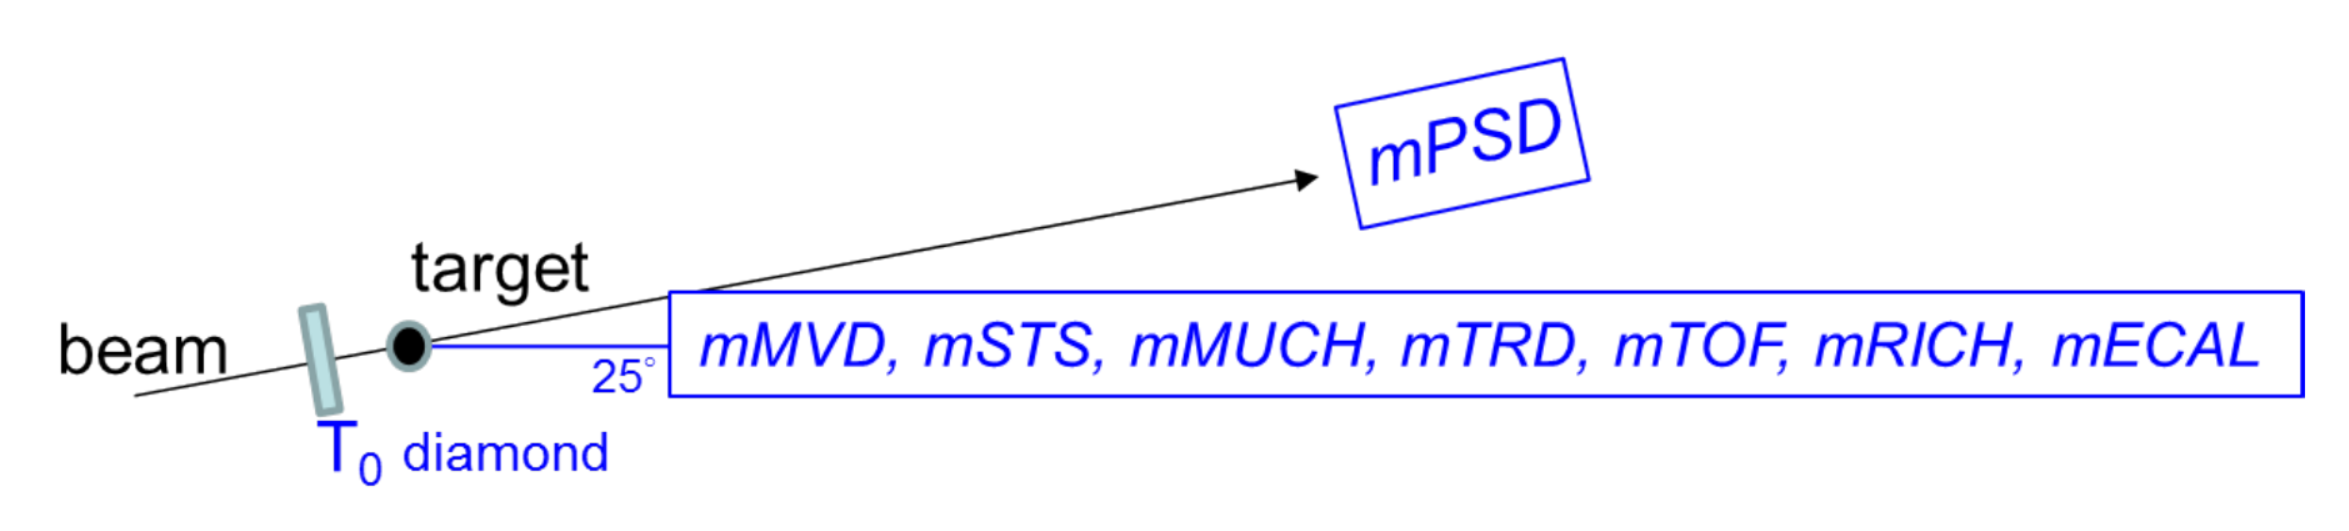
\includegraphics[width=.8\textwidth]{mCBM_sketch.png}
\caption{\label{fig:1} Concept sketch of the proposed mCBM test-setup}
\end{figure}

The mCBM setup will allow to test important aspects of CBM development: the operation of the detector prototypes in a high-rate nucleus-nucleus collision environment; the free-streaming data acquisition system including the data transport to a high-performance computer farm located in the Green IT Cube; the online track and event reconstruction as well as event selection algorithms; the offline data analysis; and the detector control system.
To make possible CBM@FAIR data collection with nucleus-nucleus collision rate up to 10MHz leading to data rate up to 1TB per second, will be used ultra-fast and radiation tolerant GBTx ASIC data aggregation unit developed at CERN. Future down-stream, the data streams are handled by Data Processing Boards (DPB) containing powerful FPGAs and are forwarded via FLES Input Selector (FLES) which performs on-line event selection. In 2020-2021 DPB and FLIB will be replaced by a prototype of the Common Readout Interface (CRI) as it foreseen in CBM experiment.\cite{1}



\section{The Projectile spectator detector design}
The CBM PSD is assembled from 46 individual modules, each forming a lead-scintillation sandwich. Schematic view and photo of a single PSD module are represented in figure~\ref{fig:2}. Light readout from each scintillator plate is provided by WLS-fibers embedded in grooves in the scintillator plates. Six consecutive scintillator tiles form a section and are connected to a single photodetector at the end of the module. The longitudinal segmentation of the modules into 10 sections ensures the uniformity of light collection along the modules. Hamamatsu MPPCs S12572-010P with active area 3$\times$3 $mm^2$ are used as photodetectors for each section of module. Thus, the entire detector accounts for 460 signal readout channels. More details about the internal structure of the modules and the whole PSD design can be found in \cite{2}.


\subsection{FEE}
Each photodetector is provided with a common reference voltage of about 70 volts, as well as individual automatic correction of the reference voltage depending on the external temperature. The temperature sensor, as well as the LED for the possibility of photoelectronic calibration of photodiodes, are placed on the FEE panel. The monitoring and data collection from all FEEs are carried out by means of the slow control system.

\begin{figure}[htbp]
\centering 
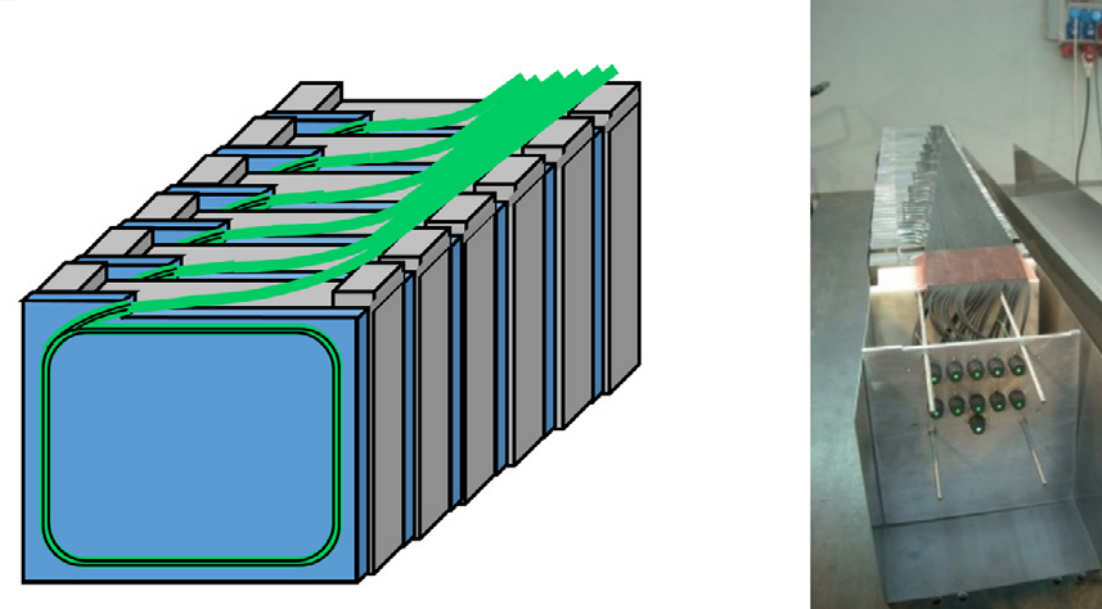
\includegraphics[width=.45\textwidth]{PSD_module.png}
\caption{\label{fig:2} Schematic view of the sampling lead/scintillator module, (left). Photo of the PSD module (right)}
\end{figure}



\section{PSD readout concept}

Signal readout is accomplished with an ADC board represented in figure~\ref{fig:3} and an Addon board represented in figure~\ref{fig:4}. Signals from MPPCs are collected by the ADC Addon board, which provides a single-ended interface based on single-ended to differential converters AD8138 ICs. Design allows for an adjustable input and output offset, utilizing the whole dynamic range of the converter. Besides providing a signal interface, Addon board includes an MPPC offset adjustment system, that consists out of 16 4-channel digital to analog converters (DACs) with unity-gain buffers. DACs provide a DC offset on the signal line, regulating voltage over the MPPC's terminals. Control of the DACs is accomplished through a STM32F103 microcontroller placed on the Addon board, which receives commands and adjustment data from the ADC board. Signal is then digitized by the ADC board designed for the ECAL detector of PANDA experiment \cite{3} (see figure~\ref{fig:3}). The 64-channel board based on ADC LTM9011 with digitization rate up to 125Msps and 14-bit digitization resolution. ADC used now in 80 Msps digitization mode, the setup will be upgraded up to 120 Msps in 2020. The ADC board is mounted directly onto the Addon board (see figure~\ref{fig:4}), and the whole assembly is designed to fit standard 6U Eurocard cradles.
Digitized samples of 64 analog signals are sent to 2 FPGAs Kintex 7 using 128 LVDS links. Each FPGA process data from 32 channels. For current tests simple signals waveform analyzing algorithm is used triggered by threshold crossing and provide charge of signal in fixed gate. An advanced signal processing algorithm based on the Prony-LS fitting procedure, which allows working with signals near the noise level, and also used for the pile-up recognition, has already been developed and will be implemented in the next tests.
To meet requirement of experiment DAQ, GBT FPGA transceiver was integrated into firmware. GBT allow to transmit data, slow control and clock. Expected data rate is 1MHz per channel that constrains 100bit/hit for GBT data rate 3.2 Gbit/s. 
LMK0460 jitter cleaner used for production ADC and MGTREF clocks. After reset 100MHz clock from on-board generator TD-100 used as master clock. After GBT RX synchronization established, source switched to external clock sourced from GBT RX. The clock switching scheme allow to maintain common DAQ clock domain. Measuring hit time in trigger-less readout occurs relative to time counting named timeslice synchronous for all experiment readout.


\begin{figure}[htbp]
	\centering
	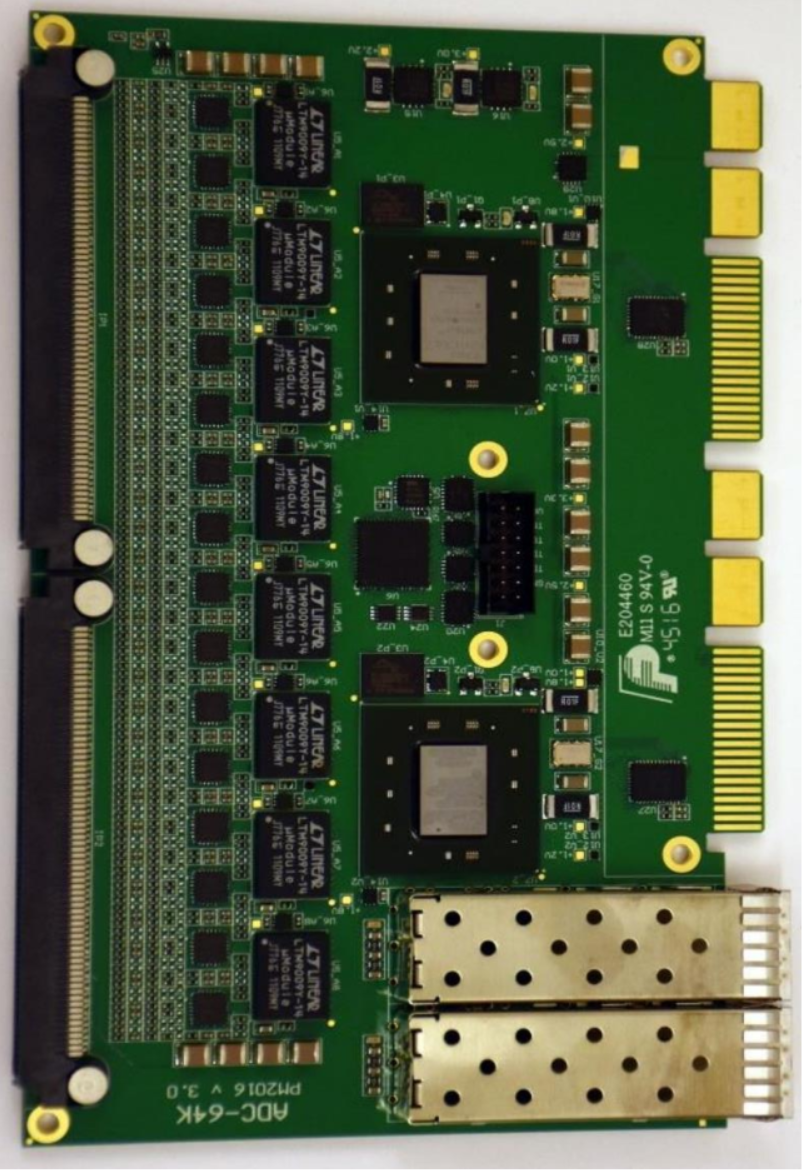
\includegraphics[width=.2\textwidth]{ADC_board.png}
	\caption{\label{fig:3} 64-channel ADC board with 2 FPGA Kintex 7}
\end{figure}

\begin{figure}[htbp]
	\centering
	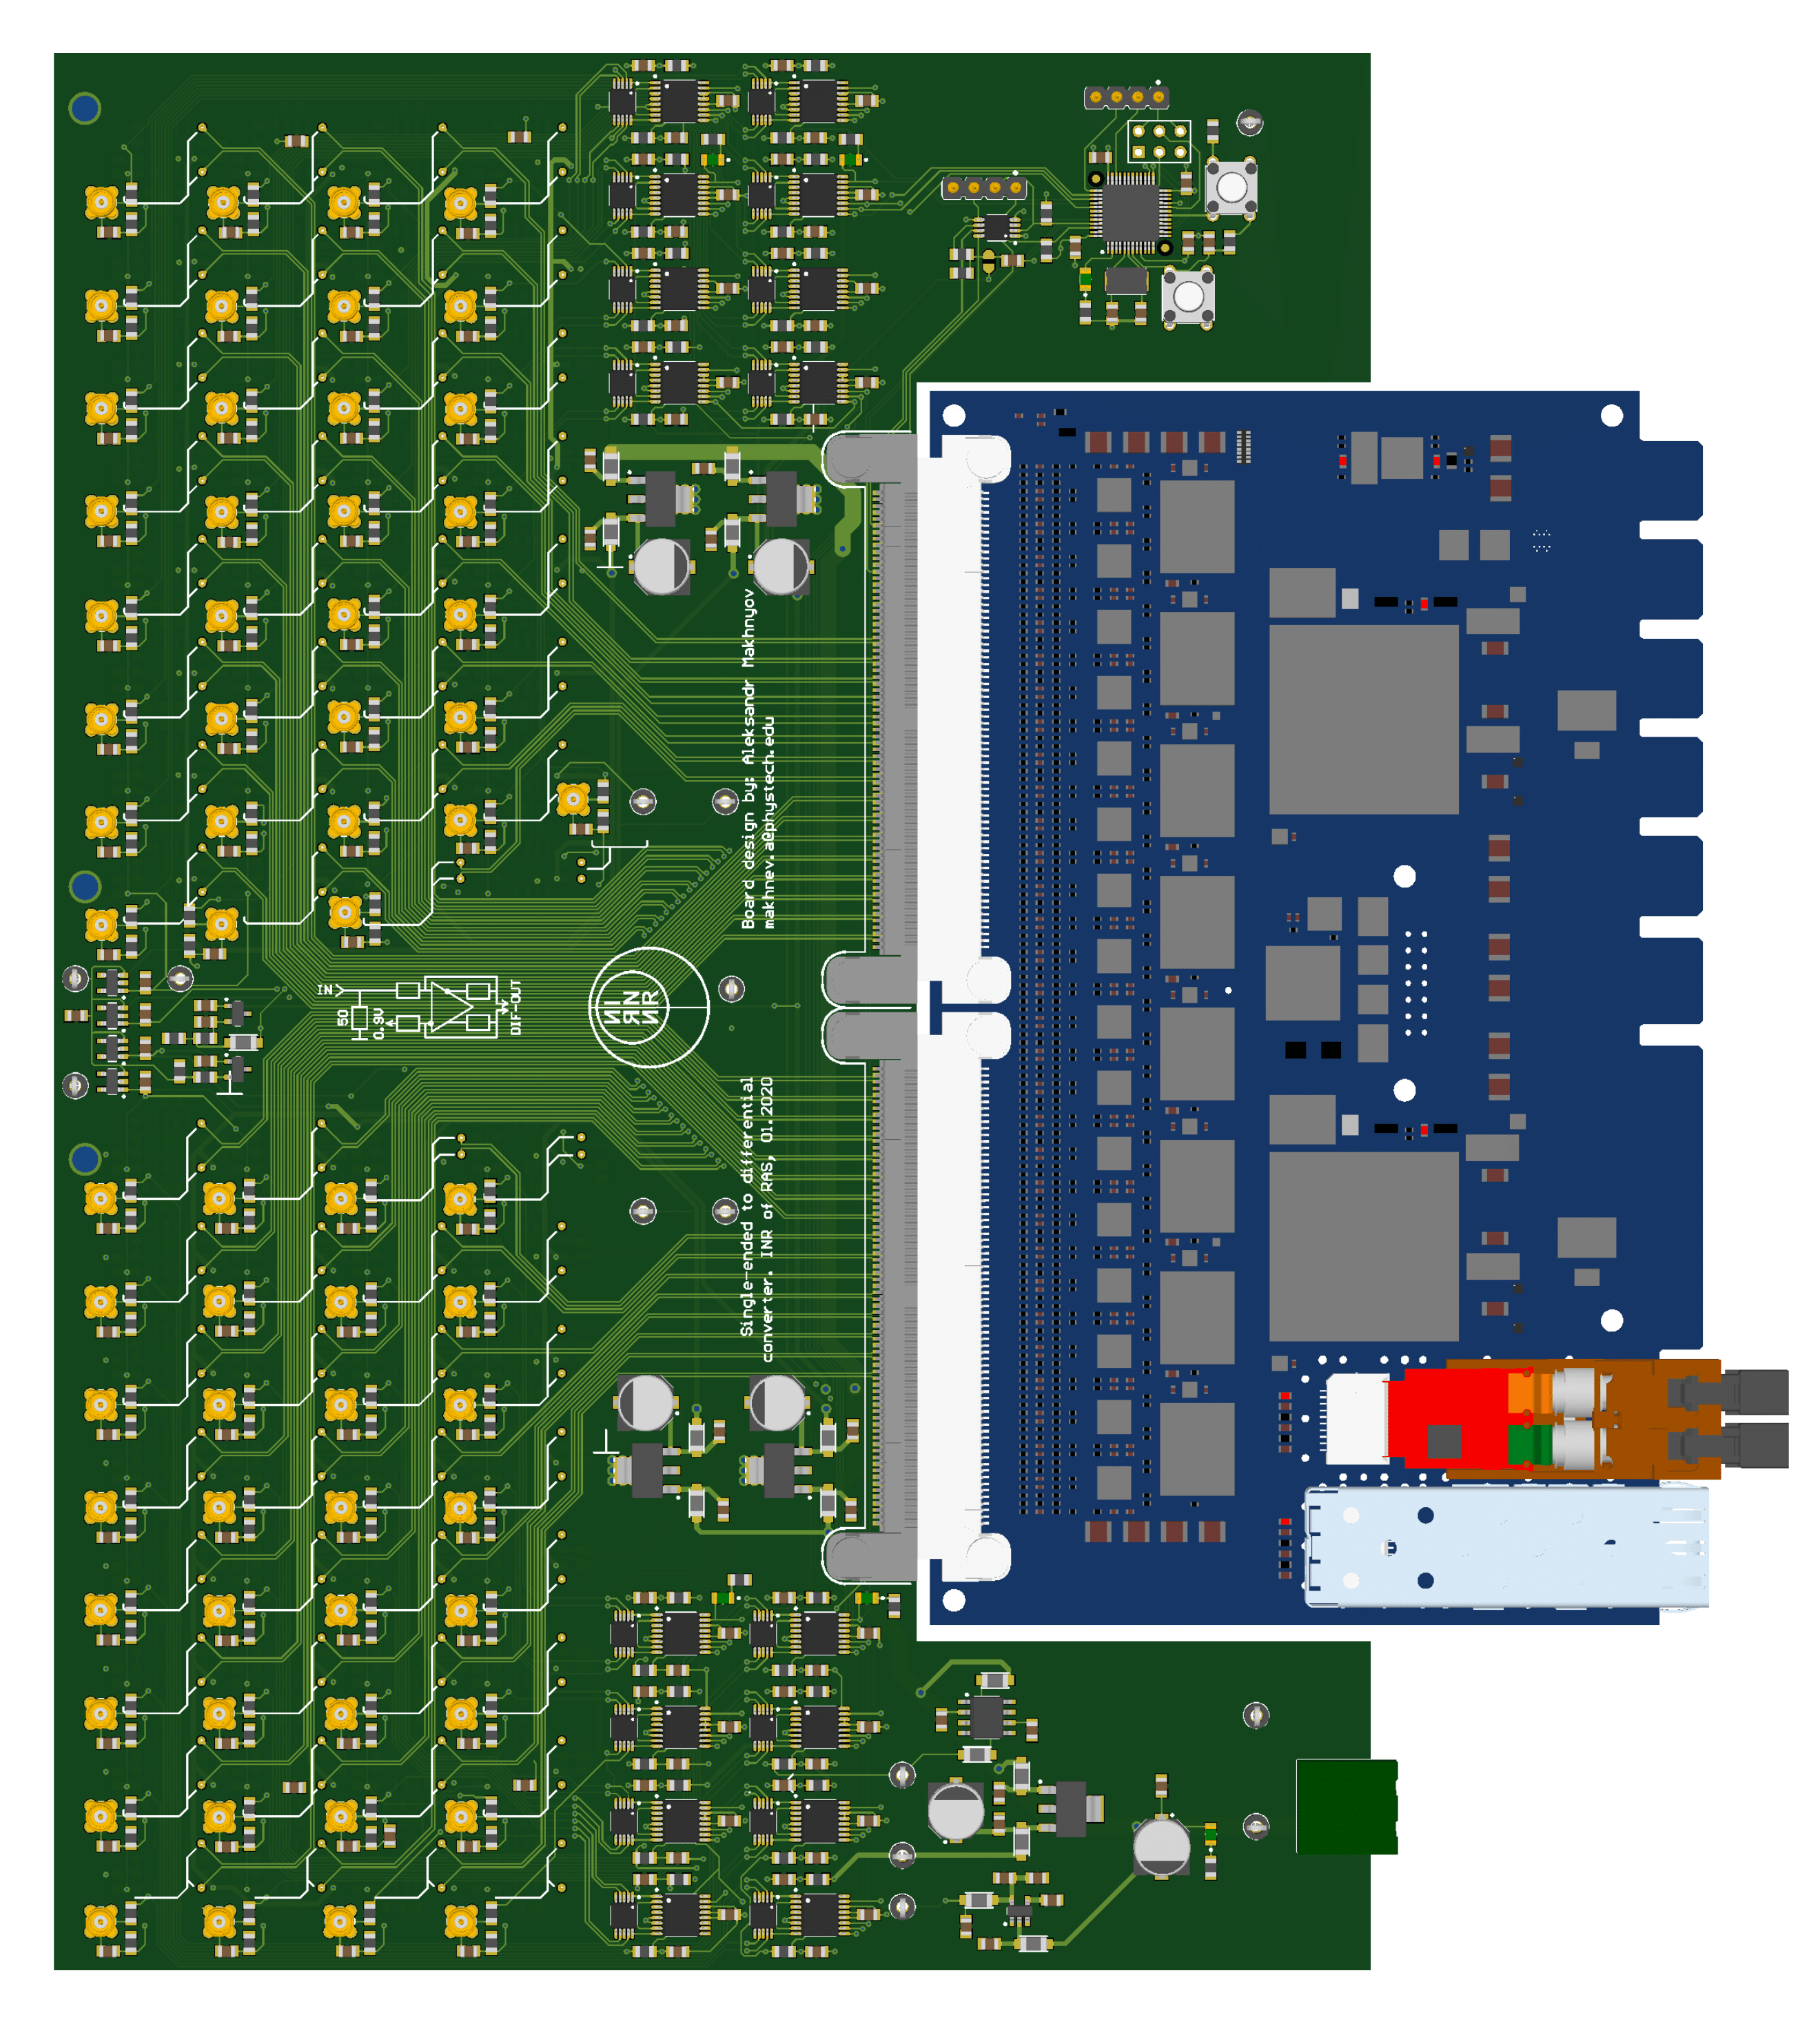
\includegraphics[width=.5\textwidth]{ADC_addon.png}
	\caption{\label{fig:4} Addon board design with the ADC board mounted}
\end{figure}

\section{PSD data monitoring}
Information of the mPSD detector is transmitted to the mCBM common data reading system using the DPB board with modified software. Currently, mPSD data packages are sets of 64-bit messages containing information about the time stamp of the signal, total number and indices of triggered channels, charges, zero levels and times of arrival of signals, as well as the information about the signal waveforms. The completeness and integrity of the received data packets is monitored by the number of read GBT words. In addition, control of all transmitted information is also carried out online through a software module for data monitoring (see figure~\ref{fig:5}). The top two graphs serve here to track the indices of triggered channels. The indices correspond to the PSD sections from 0 to 8. An external source was connected to channel 9, which serves to check the synchronization between the mCBM detectors. The lower left graph shows the distribution of energy deposition in PSD sections. The major part of the energy is deposited in the two front sections of the calorimeter. The bottom right graph shows the evolution of the length of the microslices. This information is used to verify data integrity.

\begin{figure}[htbp]
\centering % \begin{center}/\end{center} takes some additional vertical space
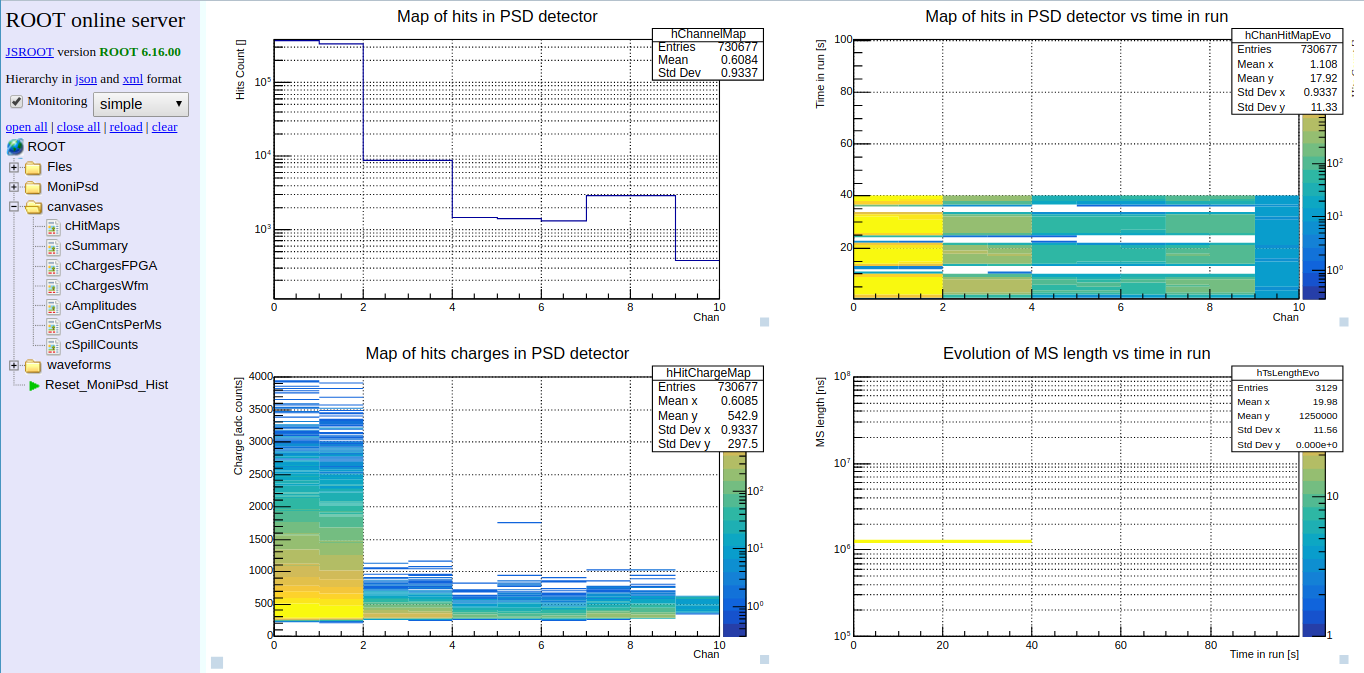
\includegraphics[width=\textwidth]{run582.png}

\caption{\label{fig:5} Data monitoring software module}
\end{figure}

\section{PSD beam data results}
During the data acquisition, information from all the detectors of the mCBM experiment is recorded in a common binary file. To check the synchronism of data from the detectors, the time correlation graphs are constructed (see figure~\ref{fig:6}). An explicit peak in the distribution of the difference in the response time of the detectors T0 and PSD, located at about 200 ns, indicates the correlation of the data and serves to select beam events.

\begin{figure}[htbp]
\centering % \begin{center}/\end{center} takes some additional vertical space
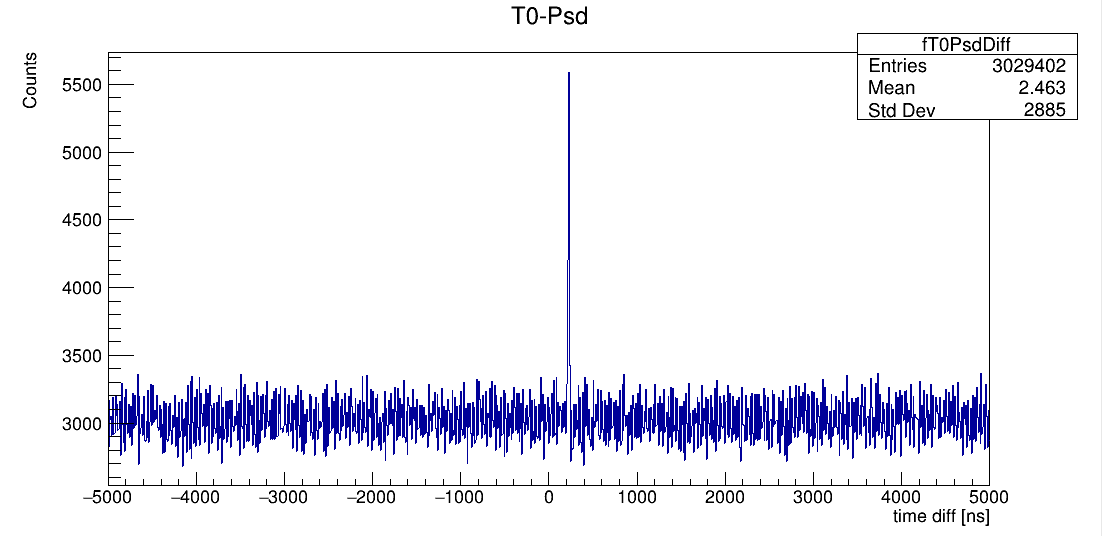
\includegraphics[width=\textwidth]{run582T0Psd.png}

\caption{\label{fig:6} T0-Psd time correlation}
\end{figure}

Since the mCBM experiment collects data in a triggerless mode, it is necessary to construct events from signals based on their time stamps while data processing. In the current approach, we assume the signals to form a single event, if their time stamps are located in a single time window of 200ns. The distribution of mPSD energy deposition in events constructed this way is shown in figure~\ref{fig:7} (left). The presence of two peaks here is explained by the discrete number of triggered sections in the event. The right side of figure~\ref{fig:7} shows the energy profile in the mPSD sections.

\begin{figure}[htbp]
\centering % \begin{center}/\end{center} takes some additional vertical space
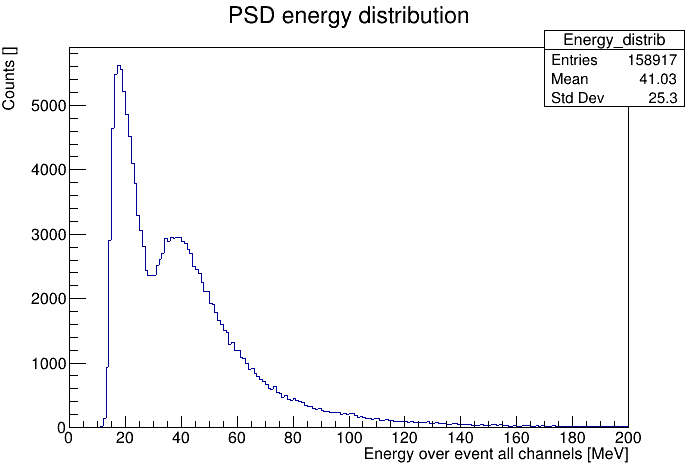
\includegraphics[width=.45\textwidth]{PsdEdepInEvent_calibrd.png}
\qquad
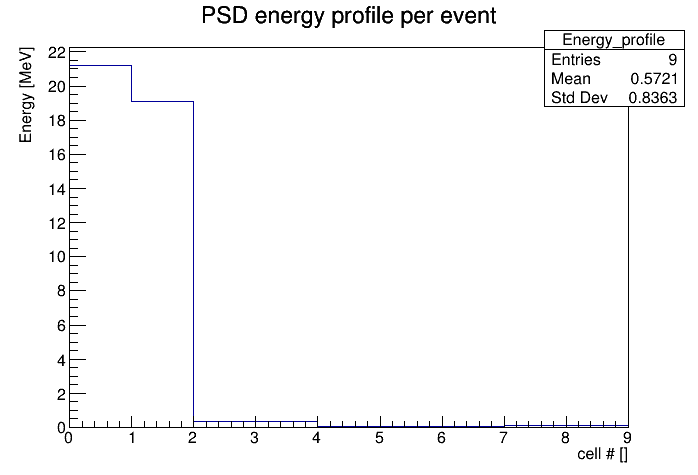
\includegraphics[width=.45\textwidth]{PsdEprofileInEvent_calibrd.png}
\caption{\label{fig:7} mPSD energy deposition (left); mPSD energy profile (right)}
\end{figure}



\acknowledgments
This work was supported by the Russian Foundation of Basic Research (RFBR) Grant No. 1



\begin{thebibliography}{99}


\bibitem{1}
\emph{A CBM full system test-setup for high-rate nucleus-nucleus collisions at GSI / FAIR} (2017) http://p31769.typo3server.info/fileadmin/fair/experiments/CBM/documents/mcbm-proposal2GPAC-WebVersion0619-SVN7729.pdf


\bibitem{2}
F.~Guber \textit{et al.} [NA61/SHINE, CBM and BM@N],
\emph{Transverse and longitudinal segmented forward hadron calorimeters with SiPMs light readout for future fixed target heavy ion experiments},
Nucl.\ Instrum.\ Meth.\ A \textbf{958} (2020), 162728
doi:10.1016/j.nima.2019.162728


\bibitem{3}
Serneguet Sorli, Á. (2015). \emph{A multichannel digitizer for the PANDA experiment.} http://hdl.handle.net/10251/56722.



\end{thebibliography}
\end{document}

